\section{Introduction}

Le mouvement respiratoire en imagerie TEP engendre plusieurs effets sur les images reconstruites, qui seront détaillés ci-après. Il occasionne notamment une diminution de la qualité des images, ce qui peut perturber le travail des praticiens. 

Nous ferons tout d'abord une introduction générale sur le mouvement respiratoire, puis nous enchaînerons ensuite sur les différents effets que peut avoir ce mouvement sur les images TEP, avec notamment des incertitudes sur la forme et la localisation des lésions et une diminution de l'activité estimée. Nous parlerons ensuite de l'impact de ce mouvement sur la détectabilité des lésions.

\section{Mouvement respiratoire}

Ce mouvement est la succession d'une phase inspiratoire, suivi d'une phase expiratoire. Chacune de ces phases combine plusieurs mouvements élémentaires~\cite{servant2007cours} :
 
\begin{enumerate}
 \item Thoracique, avec un déplacement des côtes.
 \item Abdominal, avec un déplacement du diaphragme.
 \item En cas d'inspiration forcée, action des pectoraux.
\end{enumerate}

La figure~\ref{fig:respiXCAT} représente 3 instants du cycle respiratoire utilisé dans le NCAT~\cite{segars2001These}, un modèle de corps humain respirant. On voit clairement tous les effets présentés précédemment, notamment le relèvement des côtes et du sternum par rapport aux guides de référence  présents sur les images.

\begin{figure}[h!]
    \begin{center}
            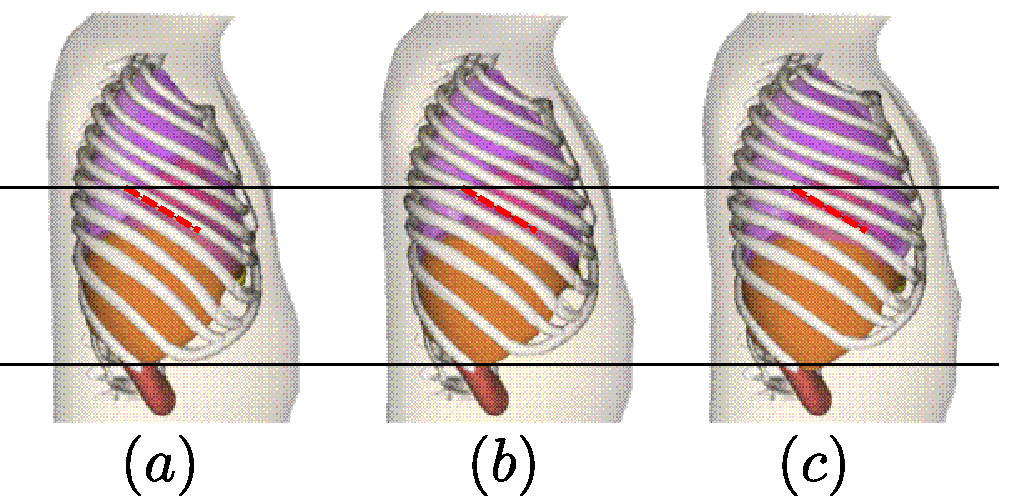
\includegraphics[width=10cm]{images/mvtRespi} \\
    \end{center}
    \caption[Modèle de mouvement intégré dans le fantôme NCAT]{Modèle de mouvement intégré dans le fantôme NCAT. La ligne pointillée rouge sert de référence pour la position d'une des côtes du modèle en expiration. L'image (a) correspond à l'expiration complète, et la (c) à la fin de l'inspiration. (b) correspond à un instant intermédiaire du cycle. }
    \label{fig:respiXCAT}
\end{figure}


La variabilité inter et intra-patient de ce mouvement est très importante : le volume d'air inspiré peut varier de 500 ml à 1200 ml selon que la personne a une respiration normale ou profonde. Pour ces deux extrêmes, la fréquence respiratoire varie de 5 cycles/min. à 20 cycles/min.~\cite{sherwood2006fundamentals}.

Or, une acquisition TEP a une durée de plusieurs minutes par lit, ce qui provoque des artefacts dûs aux mouvements réalisés pendant l'acquisition, notamment au niveau de la localisation de la tumeur, de son activité mesurée et, par extension, de sa détection. De la même manière, des artefacts (voir figure~\ref{fig:artefactsCT}) apparaissent au niveau des zones de fort mouvement dans les images TDM, lorsque les organes bougent pendant une rotation du détecteur.

Nous allons tout d'abord introduire les effets visibles sur les images, puis nous nous attarderons sur les mesures quantitatives utilisées pour étudier l'apport de la correction du mouvement sur la détection des tumeurs. Enfin, nous dresserons un état de l'art plus précis des publications s'intéressant à l'impact du mouvement respiratoire sur la détection.

\section{Localisation et volume}


La localisation et le volume apparent des tumeurs sur les images TEP peuvent être modifiés par le mouvement engendré par la respiration (voir figure~\ref{fig:effetMvt}). D'après l'étude de~\cite{lamare2007respiratory}, réalisée sur des simulations Monte-Carlo à l'aide du logiciel de simulation GATE~\cite{jan2004gate} en utilisant le modèle NCAT~\cite{segars2001These}, la largeur à mi-hauteur des lésions peut être modifiée de 48\% (équation~\ref{eq:PRD} : Différence relative) dans le cas d'une lésion de 7mm de diamètre dans la partie basse du poumon. L'imprécision axiale sur le positionnement de la tumeur peut atteindre 9\% dans les mêmes conditions.

\begin{equation}
\%DR= \left| \frac{Crit\grave{e}re~sur~image~non~corrig\acute{e}e - Crit\grave{e}re~sur~image~de~r\acute{e}f\acute{e}rence}{Crit\grave{e}re sur image~de~r\acute{e}f\acute{e}rence} \right|
\label{eq:PRD}
\end{equation}


\begin{figure}[h!]
    \begin{center}
            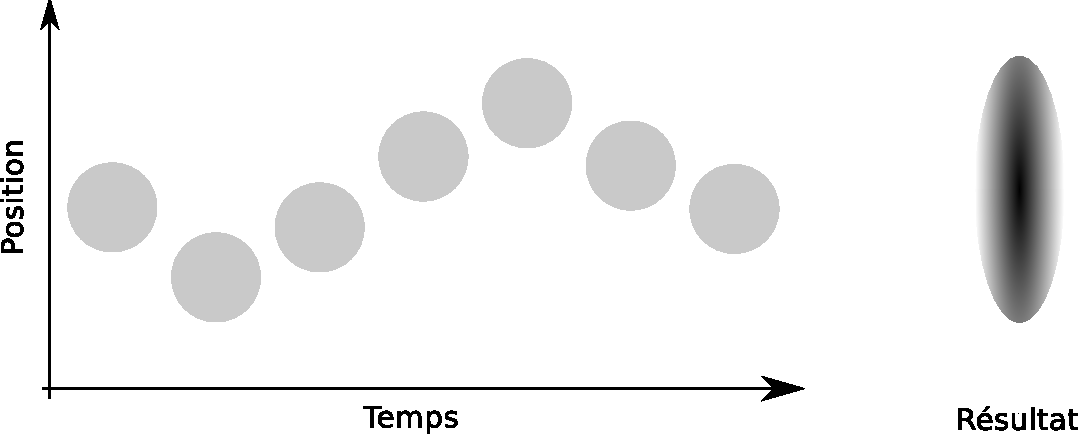
\includegraphics[width=10cm]{images/moyennageImage} \\
    \end{center}
    \caption[Effet du déplacement d'une tumeur sur les données acquises]{Effet du déplacement d'une tumeur sur les données acquises. La position de la tumeur change en fonction du temps, ce qui provoque l'acquisition d'une tumeur équivalente présentée à droite.}
    \label{fig:effetMvt}
\end{figure}


\section{Mesure de l'activité des tumeurs}

Le contraste des tumeurs par rapport au fond est un critère important pour déterminer la malignité des tumeurs~\cite{dimitrakopoulou2002role, krak2005effects}. De plus ce contraste joue aussi un rôle important sur la détectabilité de la tumeur en facilitant sa distinction du fond, comme nous allons le voir ci-après.

L'activité peut être influencée par la respiration de deux manières : 
\begin{itemize}
 \item Par un mauvais ajustement de la carte d'atténuation.
 \item Par le moyennage de la position de la tumeur.
\end{itemize}


\subsection{Décalage de la carte d'atténuation}

La carte d'atténuation utilisée pour corriger les images d'émission est basée sur une image TDM prise à un instant donné du cycle. Or l'atténuation de la zone correspondant à une tumeur peut être différente de celle des tissus environnants, ce qui peut occasionner des sous-estimations ou des sur-estimations de l'activité de la tumeur si la carte d'atténuation est mal positionnée.

D'après l'étude~\cite{erdi2004ct}, on peut observer des variations très importantes de $SUV_{max}$ (voir équation~\ref{eq:varSUV}) sur les images TEP reconstruites. L'étude a été réalisée sur 5 patients totalisant 8 lésions. L'acquisition TDM 4D a été synchronisée sur le mouvement à l'aide d'un dispositif placé sur l'abdomen du patient. Ce dispositif était constitué de deux marqueurs réfléchissant les ondes infrarouges, placés dans le champ de vue d'une caméra. Les données synchronisées acquises en TDM 4D ont été utilisées pour générer un cycle de 10 images TDM. Chacune de ces 10 images a ensuite servi de carte d'atténuation lors de la reconstruction des images d'émission, générant ainsi 10 images TEP .

\begin{equation}
\label{eq:varSUV}
 \%~variation~SUV_{max} = 100 \times \frac{ | SUV_1 - SUV_2 | }{ (SUV_1 + SUV_2) / 2 }
\end{equation}


Les données TEP reconstruites à partir des 10 images ont montré de grandes différences en terme de SUV selon l'instant du cycle à partir duquel les lésions ont été extraites.
Ces variations allant jusqu'à 24\% pour une lésion de $19.8~mm^3$ placée dans l'espace médiastinal, entre une reconstruction TEP réalisée à partir d'une image TDM de fin d'expiration et une image TDM de fin d'expiration. En recherchant la variation la plus grande sur l'ensemble du cycle (en non pas en se limitant aux extrêmes), la variation peut atteindre 30\%.

La figure~\ref{fig:lesionEnFctPhaseTDM} présente la variation de $SUV_{max}$ en fonction de la phase utilisée pour la reconstruction.


\begin{figure}[h!]
	\vspace{0.5cm}
	\centering
			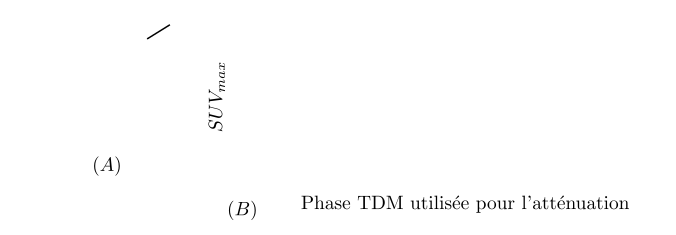
\includegraphics[width=12cm]{images/lesionEnFctPhaseTDM}
	\vspace{-0.5cm}
	\caption[Influence de l'influence de la carte d'atténuation sur l'activité des lésions] {A) Vue coronale d'un patient avec une lésion clairement visible en haut à droite (flèche noire).  B) $SUV_{max}$ observé sur les images reconstruites en fonction de l'image TDM utilisée pour la reconstruction. Le nombre en abscisse représente la position dans le cycle respiratoire en pourcentage.} 
	\label{fig:lesionEnFctPhaseTDM}
\end{figure}

\subsection{Artefacts TEP dus aux artefacts TDM}

On peut voir sur les images de la figure~\ref{fig:artefactsCT} des artefacts présents sur les images TDM utilisées pour la correction d'atténuation. Ces artefacts proviennent de la manière dont les images sont acquises : le couple ``source de rayons X-détecteur'' tourne autour du sujet dans un mouvement hélicoïdal, et l'algorithme de reconstruction va ensuite utiliser les acquisitions pour reconstruire une image complète. Or, en cas de respiration rapide, des incohérences peuvent survenir quand le mouvement du diaphragme est plus important que celui de la caméra. Ce type d'artefacts peut créer des incohérences dans les images TEP reconstruites, car le poumon sera corrigé de l'atténuation avec des coefficients non uniformes.

\begin{figure}[h!]
	\begin{center}
		\begin{tabular}{c c}
			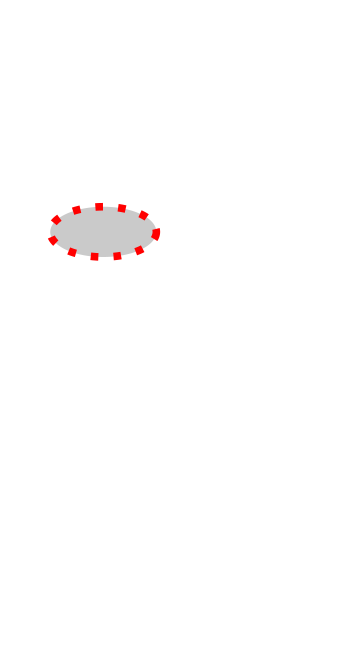
\includegraphics[width=5cm]{images/artefactCT1} & 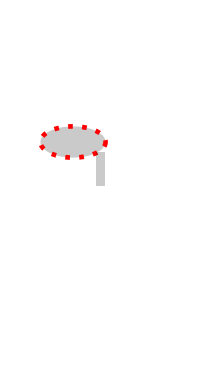
\includegraphics[width=5cm]{images/artefactCT2}
		\end{tabular}
	\end{center}
	\caption{Artefacts présents sur des images TDM utilisées pour la correction d'atténuation.} 
	\label{fig:artefactsCT}
\end{figure}


\subsection{Déplacement de la tumeur au cours du cycle}

Le mouvement respiratoire va avoir pour effet de déplacer la tumeur pendant l'acquisition, ce qui va moyenner la quantité de radioactivité sur l'ensemble du cycle, comme indiqué sur la figure~\ref{fig:effetMvt}. Si le déplacement de la tumeur est suffisamment grand par rapport à son diamètre, la réduction de radioactivité va être importante.

L'étude~\cite{boucher2004respiratory} réalisée sur un fantôme elliptique (modèle ``Elliptical Jaszczak Phantom'') montre qu'un déplacement d'une source radioactive de 6 mm sur un cycle respiratoire moyen entraîne une sous-estimation de l'activité maximale de la source de 41\% pour un objet de 1.2 ml et de 21\% pour une sphère de 19.4 ml.


\section{Impact du mouvement respiratoire sur la détection}

Peu de travaux ont été réalisés sur l'impact du mouvement respiratoire sur la détection des tumeurs. Globalement, les publications traitent  principalement de la mesure de la quantification des lésions ($SUV_{max}$, profils de lésions, ...). Très peu d'articles utilisent des critères orientés sur les performance de détection.

Voici une liste des critères utilisés dans différentes publications pour évaluer les performances d'algorithmes de correction du mouvement respiratoire :

\begin{enumerate}
 \item Basés sur la récupération de l'activité des lésions, $SUV_{max}$, contraste :~\cite{GuopingChang2010Implementation,lamare2007list,nehmeh2002effect,detorie2008quantitative}.
 \item Sur la visualisation des profils de lésion :~\cite{GuopingChang2010Implementation,Thielemans2006Lesion,lamare2007list}.
 \item Sur la récupération du volume et de la position de la lésion :~\cite{GuopingChang2010Implementation,lamare2007list,nehmeh2002effect}.
 \item Sur le rapport signal sur bruit (SNR) :~\cite{GuopingChang2010Implementation}.
 \item Sur l'observateur de Hotelling (CHO) :~\cite{Thielemans2006Lesion}.
\end{enumerate}

Comme on peut le voir, les deux seuls critères qui pourraient s'approcher d'une étude sur la détection sont le SNR et le CHO, mais ils sont largement sous-représentés. 

Je vais me concentrer sur les deux publications the Thielemans et Chang qui utilisent un observateur.

Un autre document par Rahmim Arman~\cite{rahmim4d} propose d'utiliser le CHO pour évaluer l'amélioration de la détection des défauts dans de l'imagerie cardiaque corrigée du mouvement respiratoire. Ce document n'a pas encore donné lieu à publication.
	
\subsection{Article de Thielemans et al.~\cite{Thielemans2006Lesion}}
\label{lab:articleThielPres}
Dans sa publication, Thielemans et al. utilisent le ``Channelized Hotelling Observer'' (CHO)~\cite{barrett1993model}, qui est un observateur dérivé du classifieur linéaire LDA présenté en \ref{lab:LDA}, utilisé en conjonction avec des informations fréquentielles. 

L'étude se base sur des simulations analytiques d'un fantôme thoracique dans lequel sont insérées des lésions sphériques de gros diamètre (13 mm) et de contraste élevé (4.25:1). Cette étude qui compare plusieurs méthodes de correction du mouvement respiratoire est détaillée dans le chapitre suivant en~\ref{lab:evolGating}.
%
%Cependant ils n'utilisent le CHO que sur des lésions de forts diamètre et de fort contraste (13mm de diamètre et contraste de 4.25:1).


%Les résultats présentés (figure~\ref{fig:apportCHO}) montrent une amélioration du score pour les méthodes de correction de l'ordre de 50\% dans certains cas. 

%Mais il est difficile d'évaluer de manière précise l'apport des méthodes de détection à l'aide de ces seuls ``scores'' car ce sont des résultats qualitatifs. 



\subsection{Article de Chang et al.~\cite{GuopingChang2010Implementation}}

Cette publication est une évaluation clinique d'un système de découpage automatique du signal respiratoire selon l'amplitude. Elle est basée sur 13 patients totalisant 21 tumeurs du poumon de taille diverses (estimée de 1 à 27 cm$^3$. Le signal respiratoire est acquis à l'aide d'un dispositif propriétaire (Anzai AZ-733V) basé sur une ceinture abdominale avec capteur de pression. Seules les données TEP acquises autour d'une amplitude présélectionnée (+/-10\% de l'amplitude correspondant à l'acquisition TDM) sont utilisées pour la reconstruction des images corrigées. 

Le jeu d'images ``témoin'', non corrigées, est réalisé en extrayant des données acquises le même nombre d'évènements N que le jeu d'images synchronisées en considérant les N premiers du fichier en mode séquentiel.

L'auteur compare le $SUV_{max}$, $SUV_{moyen}$, Rapport Signal/Bruit (SNR) et volume apparent de la lésion pour les deux jeux d'images. Le volume de la lésion et le $SUV _{moyen}$ sont calculés sur une région d'intérêt correspondant à 40\% du $SUV_{max}$ de la lésion. Le SNR est calculé en divisant le SUV moyen de la tumeur par l'écart-type d'une zone d'intérêt dans le poumon, dont ni la taille ni la localisation ne sont précisées. 

Les résultats présentés montrent une amélioration importante des valeurs du SNR pour les images corrigées du mouvement par rapport aux images témoin, comme présenté dans la figure~\ref{fig:guoping2010Exemple}. En moyenne, cette augmentation est de 26.3\%, mais deux tumeurs sur les 21 de l'étude voient leur SNR augmenter de plus de 66\%. 

\begin{figure}[h!]
	\centering
			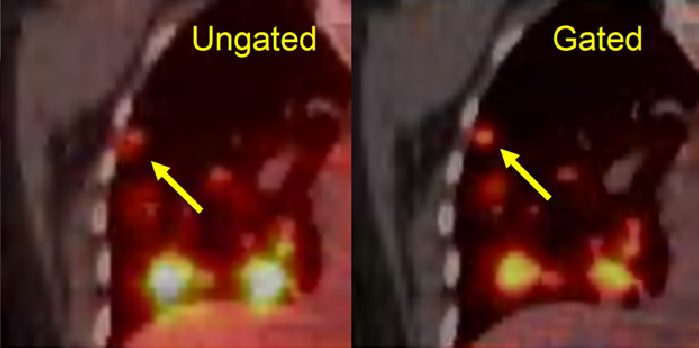
\includegraphics[width=10cm]{images/guoping2010Exemple}
	\caption{Exemple d'image avec et sans correction de mouvement respiratoire.} 
	\label{fig:guoping2010Exemple}
\end{figure}




Il est étonnant de constater que les mesures moyennes sur les 21 tumeurs de $SUV_{max}$ et $SUV_{moyen}$ voient leurs valeurs augmenter respectivement de 26.8\% et 26\%, ce qui est tout à fait semblable avec l'augmentation de SNR. Cependant, les valeurs individuelles d'amélioration  pour chaque tumeur ne montrent pas de corrélation avec le SNR. Par exemple, une lésion va montrer une augmentation de 24\% de son $SUV_{max}$, de 20\% de son $SUV_{moyen}$ et de 37\% de son SNR.

Il est intéressant de constater qu'il y a un point où le SNR diminue de 3.4\%, mais que le $SUV_{max}$ et le $SUV_{moyen}$ augmentent tout de même de presque 18\%. Cela semble indiquer une erreur car le SUV de la zone d'intérêt n'est pas censé changer de manière importante.
